\section{Experiment}

Once again, we are focusing on the context switching time.
We used the same application described in section \ref{sec:internal-experiment}.
The application contains two tasks that wait 1ms on run one after the other.

\subsection{Reference value}

The reference value for the context switching time is the same measured in the section \ref{sec:reference-value}.
No changes was needed for this reference measurement as, once again, we are trying to retrieve the context switching time with our external benchmarking.

\subsection{Methodology}

Our first idea to develop this external framework was to implement it with Python3.7 on a desktop computer.
Using the UART protocol over USB, the board sends a single byte containing the process ID that is read by a Python script on the computer.

The motivations for using this alternative are:
\begin{itemize}
  \item Sending one byte of data over USB with UART have a smaller impact than computing the context switching time locally on the board;
  \item Heavy computational tasks of the framework are done on the computer and not on the board;
  \item Using Python3.7, we can achieve a time precision at the nanosecond.
\end{itemize}

However, after discussing with the embedded community, we abandonned this idea for the following reasons.
There is buffering happening on the USB-serial chip on the board, on the PC's USB hardware, in the PC USB-serial driver and also in the desktop operating systems.
Those buffering will add delay in our measurements.
Context switching will occur on the desktop computer that will invalidate any timing value.

Instead, we decided to use a device called the Pocket Science Lab to perform our experiment.


\begin{figure}[!ht]
  \centering
  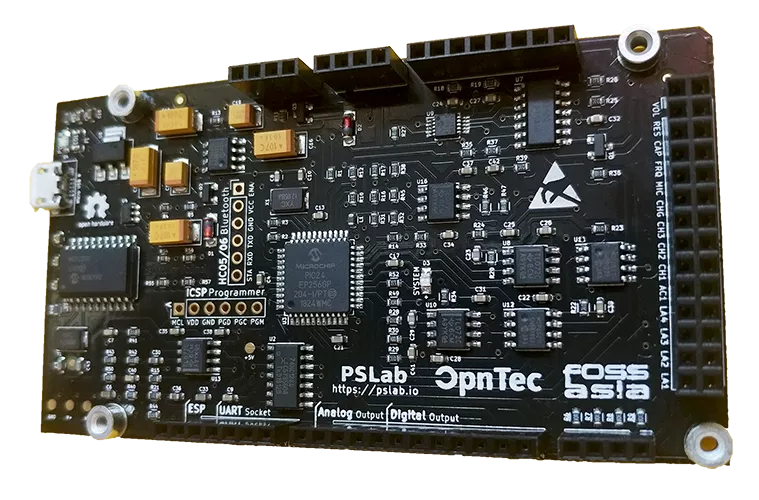
\includegraphics[scale=0.25]{assets/pslab.png}
  \caption{\label{fig:pslab}Pocket Science Lab device from \href{https://pslab.io}{PSLab.io}}
\end{figure}

\paragraph{PSLab}
The Pocket Science Lab device from \href{https://pslab.io}{PSLab.io} comes with a built-in 4-Channel up to 2MSPS oscilloscope, multimeter, 4-Channel, 4 MHz logic analyser, and other digital instruments.
Using the Python librairy \href{https://github.com/fossasia/pslab-python}{pslab-python}, we can communicate with the board and experiment with it.

\subsubsection{Framework implementation}



\subsection{Experiment setup}
For this second experiment, we used the same Zolertia RE-MOTE board described in section \ref{sec:internal-setup}.

The Python3 script was run under Linux on a quad-core laptop computer.